% =============================================================================
% Template baseado no padrao IComp/UFAM (abntex2)
% Atividade: Comunicacao sem fio -- da informacao ao canal
% Medicao de vazao em rede Wi-Fi com ESP32 e Wireshark
% =============================================================================
\documentclass[
  12pt,
  a4paper,
  oneside,
  brazil,
  chapter=TITLE,
  section=TITLE,
]{abntex2}

% -- Pacotes -------------------------------------------------------------------
\usepackage[T1]{fontenc}
\usepackage[utf8]{inputenc}
\usepackage[brazil]{babel}
\usepackage{times}
\usepackage{microtype}
\usepackage{amsmath,amssymb}
\usepackage{graphicx}
\usepackage{xcolor}
\usepackage{booktabs}
\usepackage{caption}
\usepackage{subcaption}
\usepackage{listings}
\usepackage{float}
\usepackage{enumitem}
\usepackage{indentfirst}
\usepackage{siunitx}
\usepackage{array}
\usepackage{abntex2cite}
\usepackage{hyperref}

\sisetup{output-decimal-marker={,}, group-separator={.}, group-minimum-digits=4}

\definecolor{ufamblue}{RGB}{0,51,102}
\definecolor{codegreen}{rgb}{0,0.45,0}
\definecolor{codegray}{rgb}{0.5,0.5,0.5}
\definecolor{codeblue}{rgb}{0.1,0.1,0.65}
\definecolor{backcolour}{rgb}{0.97,0.97,0.97}

\lstdefinestyle{cpp}{
  language=C++,
  backgroundcolor=\color{backcolour},
  commentstyle=\color{codegreen}\itshape,
  keywordstyle=\color{codeblue}\bfseries,
  numberstyle=\tiny\color{codegray},
  stringstyle=\color{orange!80!black},
  basicstyle=\ttfamily\scriptsize,
  breaklines=true, keepspaces=true,
  numbers=left, numbersep=6pt,
  frame=single, framerule=0.4pt,
  rulecolor=\color{gray!50}, tabsize=2,
}

\hypersetup{
  colorlinks=true,
  linkcolor=ufamblue,
  urlcolor=ufamblue,
  citecolor=ufamblue,
  pdftitle={Comunicacao sem fio: da informacao ao canal},
  pdfauthor={Matheus Serrao Uchoa},
}

% -- Metadados abntex2 ---------------------------------------------------------
\titulo{Comunicação sem fio: da informação ao canal\\Medição de Vazão em Rede Wi-Fi com ESP32 e Wireshark}
\autor{Matheus Serrão Uchôa}
\local{Manaus -- AM}
\data{\the\year}
\orientador{Prof. Celso Barbosa Carvalho}
\instituicao{%
  Universidade Federal do Amazonas -- UFAM\\
  Instituto de Computação\\
  Disciplina: Redes Sem Fio
}
\tipotrabalho{Relatório Técnico}
\preambulo{Relatório técnico apresentado à disciplina de Redes Sem Fio do
Instituto de Computação da Universidade Federal do Amazonas (UFAM), como
requisito parcial de avaliação.}

% =============================================================================
\begin{document}
% =============================================================================
\frenchspacing

% -- CAPA ----------------------------------------------------------------------
\begin{capa}
  \center
  
\includegraphics[width=3.8cm]{../mestrado_ppgee/ufam_logo.png}\\[6pt]
  {\large\bfseries\MakeUppercase{Universidade Federal do Amazonas}}\\[2pt]
  {\normalsize Instituto de Computação}\\[2pt]
  {\normalsize Disciplina: Redes Sem Fio}\\[50pt]

  {\ABNTEXchapterfont\large\MakeUppercase{\imprimirtitulo}}

  \vfill
  {\large\imprimirautor}\\[6pt]
  {\small maktheus@gmail.com}
  \vfill
  {\normalsize\imprimirlocal}\\
  {\normalsize\imprimirdata}
\end{capa}

% -- FOLHA DE ROSTO ------------------------------------------------------------
\begin{folhaderosto}
  \begin{center}
    {\large\bfseries\MakeUppercase{\imprimirautor}}\\[40pt]
    {\ABNTEXchapterfont\large\MakeUppercase{\imprimirtitulo}}\\[40pt]
  \end{center}
  \hspace{.45\textwidth}
  \begin{minipage}{.5\textwidth}
    \imprimirpreambulo\\[8pt]
    \textbf{Professor:} \imprimirorientador
  \end{minipage}
  \vfill
  \begin{center}
    {\normalsize\imprimirlocal}\\
    {\normalsize\imprimirdata}
  \end{center}
\end{folhaderosto}

% -- RESUMO --------------------------------------------------------------------
\begin{resumo}
Este relatório aborda os conceitos fundamentais que determinam a capacidade de
transmissão de um sistema sem fio --- taxa da fonte, taxa do canal, modulação
digital e capacidade --- e os relaciona a um experimento prático de medição de
vazão (\textit{throughput}) em rede Wi-Fi. Um \textit{firmware} para a
plataforma ESP32 foi desenvolvido para transmitir pacotes UDP com tamanho e
intervalo configuráveis, enquanto a vazão efetiva foi medida no computador
receptor com o analisador de protocolos Wireshark (filtro
\texttt{udp.port == 5000}). Foram avaliadas a influência do tamanho do pacote
(Tabela~A), do intervalo entre transmissões (Tabela~B) e da distância
(Tabela~C, opcional). Os resultados mostram que a taxa medida fica
sistematicamente abaixo da taxa teórica da fonte devido ao \textit{overhead} de
protocolo, ao limite de processamento do ESP32 e às perdas em alta carga, sendo
o \textbf{intervalo entre pacotes} o parâmetro de maior impacto sobre a vazão,
pois é ele que leva o sistema à saturação. Conclui-se que a vazão útil de um
enlace Wi-Fi é governada pela relação entre a taxa gerada pela fonte e a
capacidade do canal, esta última dependente da modulação adaptativa e da
qualidade do sinal (SNR).

\vspace{\onelineskip}
\noindent\textbf{Palavras-chave:} Comunicação sem fio. Wi-Fi. Vazão. ESP32.
UDP. Wireshark. Modulação digital. Capacidade de canal.
\end{resumo}

% -- SUMARIO -------------------------------------------------------------------
\pdfbookmark[0]{\contentsname}{toc}
\tableofcontents*
\cleardoublepage

% =============================================================================
\textual
% =============================================================================

% -- 1. INTRODUCAO -------------------------------------------------------------
\chapter{Introdução}

Toda comunicação digital começa com a geração de informação por uma aplicação.
Seja um sensor de temperatura, um sensor de umidade, um fluxo de áudio, vídeo ou
dados industriais, a informação é sempre convertida em \textbf{bits} antes de
ser transmitida. A quantidade de bits produzida por unidade de tempo é a
\textbf{taxa da fonte}; a quantidade de bits que o meio físico consegue
transportar é a \textbf{taxa do canal}. Quando a primeira supera a segunda,
surgem perdas e atrasos \cite{tanenbaum2011}.

Um sistema de comunicação pode ser representado pelos blocos
\emph{fonte de informação $\rightarrow$ transmissor $\rightarrow$ canal
$\rightarrow$ receptor $\rightarrow$ destino}. O transmissor não envia bits
diretamente pelo ar: ele converte a sequência binária em um sinal
eletromagnético por meio da \textbf{modulação digital}, alterando amplitude,
frequência ou fase de uma portadora \cite{proakis2007}. A escolha da modulação
influencia diretamente a taxa de transmissão e a robustez a ruído e
interferência.

Este relatório apresenta esses conceitos e os verifica experimentalmente: um
ESP32 transmite pacotes UDP por uma rede Wi-Fi e a vazão efetiva é medida no
computador receptor com o Wireshark, variando-se o tamanho do pacote, o
intervalo entre transmissões e a distância.

% -- 2. OBJETIVOS --------------------------------------------------------------
\chapter{Objetivos}

\section{Objetivo Geral}
Compreender, de forma teórica e experimental, a relação entre a taxa da fonte e
a vazão efetivamente observada em uma rede Wi-Fi, utilizando ESP32 como
transmissor e Wireshark como instrumento de medição.

\section{Objetivos Específicos}
\begin{enumerate}[label=\alph*)]
  \item compreender a relação entre taxa da fonte e taxa observada na rede;
  \item avaliar o impacto do tamanho do pacote UDP sobre a vazão;
  \item avaliar o impacto do intervalo entre transmissões;
  \item avaliar o impacto da distância entre transmissor e receptor;
  \item utilizar o Wireshark para medir o tráfego de rede (pacotes, bytes e
        \textit{throughput} médio).
\end{enumerate}

% -- 3. FUNDAMENTACAO TEORICA --------------------------------------------------
\chapter{Fundamentação Teórica}

\section{Taxa da fonte}
A taxa da fonte $R_f$ representa a quantidade de informação produzida pela
aplicação por unidade de tempo:
\begin{equation}
  R_f = \frac{\text{bits gerados}}{\text{segundo}}.
\end{equation}
Por exemplo, um sensor que envia \SI{100}{bytes} por segundo gera
$100 \times 8 = \SI{800}{bps}$. Nem toda aplicação exige altas taxas, conforme a
Tabela~\ref{tab:fontes}.

\begin{table}[H]
  \centering
  \caption{Taxas típicas de fonte por aplicação.}
  \label{tab:fontes}
  \begin{tabular}{ll}
    \toprule
    \textbf{Aplicação} & \textbf{Taxa típica} \\
    \midrule
    Temperatura     & dezenas a centenas de bps \\
    Sensores IoT    & kbps \\
    Áudio           & centenas de kbps \\
    Vídeo HD        & Mbps \\
    Vídeo 4K        & dezenas de Mbps \\
    \bottomrule
  \end{tabular}
\end{table}

\section{O canal de comunicação}
O canal é o meio físico que transporta a informação (cabo Ethernet, fibra
óptica, Wi-Fi, Bluetooth, LoRa). Todo canal possui capacidade limitada. Uma
analogia útil é a hidráulica: os bits são a água, o canal é o cano e a taxa de
transmissão é a vazão. Um cano estreito limita a água transportada, assim como
um canal limita os bits transportados. Quando a taxa da fonte supera a
capacidade do canal, há acúmulo, perdas e atraso.

\section{Modulação digital}
A modulação altera características da portadora para representar bits. A
Figura~\ref{fig:constelacoes} mostra os diagramas de constelação das modulações
empregadas no Wi-Fi.

\begin{figure}[H]
  \centering
  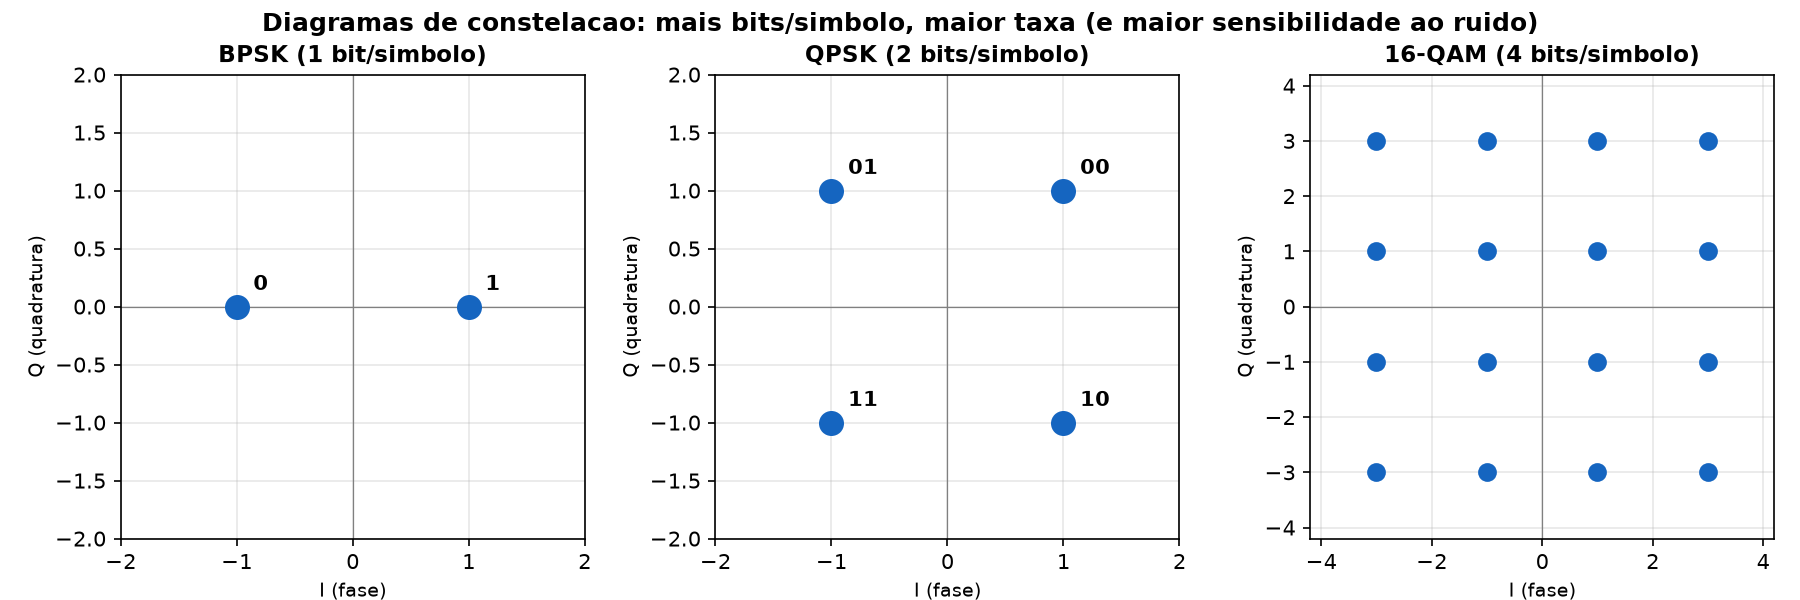
\includegraphics[width=\textwidth]{images/constelacoes.png}
  \caption{Constelações BPSK, QPSK e 16-QAM. Quanto mais pontos, mais bits por
  símbolo --- e menor a distância entre símbolos, o que aumenta a sensibilidade
  ao ruído.}
  \label{fig:constelacoes}
\end{figure}

\begin{itemize}
  \item \textbf{BPSK}: 1 bit/símbolo ($0\rightarrow 0^\circ$,
        $1\rightarrow 180^\circ$); alta robustez ao ruído, menor eficiência
        espectral.
  \item \textbf{QPSK}: 2 bits/símbolo (00, 01, 10, 11); o dobro da eficiência da
        BPSK, boa robustez.
  \item \textbf{QAM}: aumenta o número de símbolos --- 16-QAM (4 bits/símbolo),
        64-QAM (6 bits/símbolo), 256-QAM (8 bits/símbolo). Maior taxa, porém
        maior sensibilidade ao ruído.
\end{itemize}

\section{Taxa do canal e eficiência espectral}
A taxa do canal pode ser estimada por
\begin{equation}
  R_c = R_s \times b,
  \label{eq:taxacanal}
\end{equation}
onde $R_s$ é a taxa de símbolos e $b$ o número de bits por símbolo. Por exemplo,
\SI{1}{Msímbolo/s} com 64-QAM ($b=6$) resulta em $1\,\text{M} \times 6 =
\SI{6}{Mbps}$. A eficiência espectral mede quantos bits podem ser transmitidos
por símbolo: quanto maior a ordem da modulação, maior a taxa, porém maior a
exigência de qualidade do canal.

\section{Distância, SNR e adaptação de modulação}
O aumento da distância reduz a potência recebida, reduzindo a relação
sinal-ruído (SNR) e elevando a probabilidade de erro. Por isso os dispositivos
Wi-Fi empregam \textbf{adaptação automática de taxa}: canal bom $\rightarrow$
256-QAM; canal intermediário $\rightarrow$ 64-QAM; canal ruim $\rightarrow$
QPSK ou BPSK. O objetivo é manter a comunicação estável, ainda que a uma taxa
menor \cite{perahia2013,rappaport2002}.

% -- 4. METODOLOGIA ------------------------------------------------------------
\chapter{Metodologia}

\section{Ambiente experimental}
\begin{table}[H]
  \centering
  \caption{Descrição do ambiente experimental.}
  \label{tab:ambiente}
  \begin{tabular}{ll}
    \toprule
    \textbf{Item} & \textbf{Especificação} \\
    \midrule
    Transmissor (ESP32) & ESP32-WROOM-32 (DevKit~v1), Wi-Fi 802.11b/g/n 2,4\,GHz \\
    Receptor (notebook) & Notebook com interface Wi-Fi 802.11ac, Windows~11 \\
    Roteador            & Roteador doméstico 802.11n/ac, banda 2,4\,GHz, canal~6 \\
    Software de medição & Wireshark + Npcap \\
    Protocolo           & UDP, porta de destino 5000 \\
    \bottomrule
  \end{tabular}
\end{table}

\noindent\textit{Observação:} os campos da Tabela~\ref{tab:ambiente} devem ser
ajustados ao equipamento efetivamente utilizado pelo aluno.

\section{Firmware do ESP32}
O ESP32 conecta-se à rede Wi-Fi e dispara pacotes UDP em rajada contínua para o
IP do notebook. O tamanho do pacote (\texttt{TAMANHO\_PACOTE}) e o intervalo
entre transmissões (\texttt{INTERVALO\_US}) são parâmetros configuráveis; o
byte~0 de cada pacote carrega um contador de sequência para estimar perdas. O
trecho principal é mostrado a seguir (código completo em
\texttt{medicoes\_udp.ino}).

\begin{lstlisting}[style=cpp,caption={Laço de transmissão UDP do ESP32.}]
uint32_t agora = micros();
if ((int32_t)(agora - proximaTx) >= 0) {
  buffer[0] = seq++;                          // marca de sequencia
  udp.beginPacket(IP_DESTINO, PORTA_DESTINO);
  udp.write(buffer, TAMANHO_PACOTE);
  udp.endPacket();
  totalPacotes++;
  proximaTx += INTERVALO_US;                  // agenda proxima TX
}
\end{lstlisting}

A taxa teórica gerada pela fonte (apenas \textit{payload}) é
\begin{equation}
  R_f = \frac{\text{TAMANHO\_PACOTE} \times 8}{\text{INTERVALO\_US}\times 10^{-6}}.
  \label{eq:rf}
\end{equation}
Para \SI{1000}{bytes} a cada \SI{4000}{\micro\second}:
$R_f = \frac{1000\times 8}{0{,}004} = \SI{2.0}{Mbps}$.

\section{Medição com Wireshark}
Após instalar o Wireshark (e o Npcap no Windows), captura-se na interface Wi-Fi
e aplica-se o filtro de exibição \texttt{udp.port == 5000}. A vazão é obtida
em \textit{Statistics}:
\begin{itemize}[noitemsep]
  \item \textbf{Capture file properties}: número de pacotes, número de bytes e
        \textit{average bits/s};
  \item \textbf{I/O Graphs}: gráfico do \textit{throughput} ao longo do tempo
        (Figura~\ref{fig:iograph});
  \item \textbf{Conversations / Endpoints}: tráfego por par de hosts.
\end{itemize}

\begin{figure}[H]
  \centering
  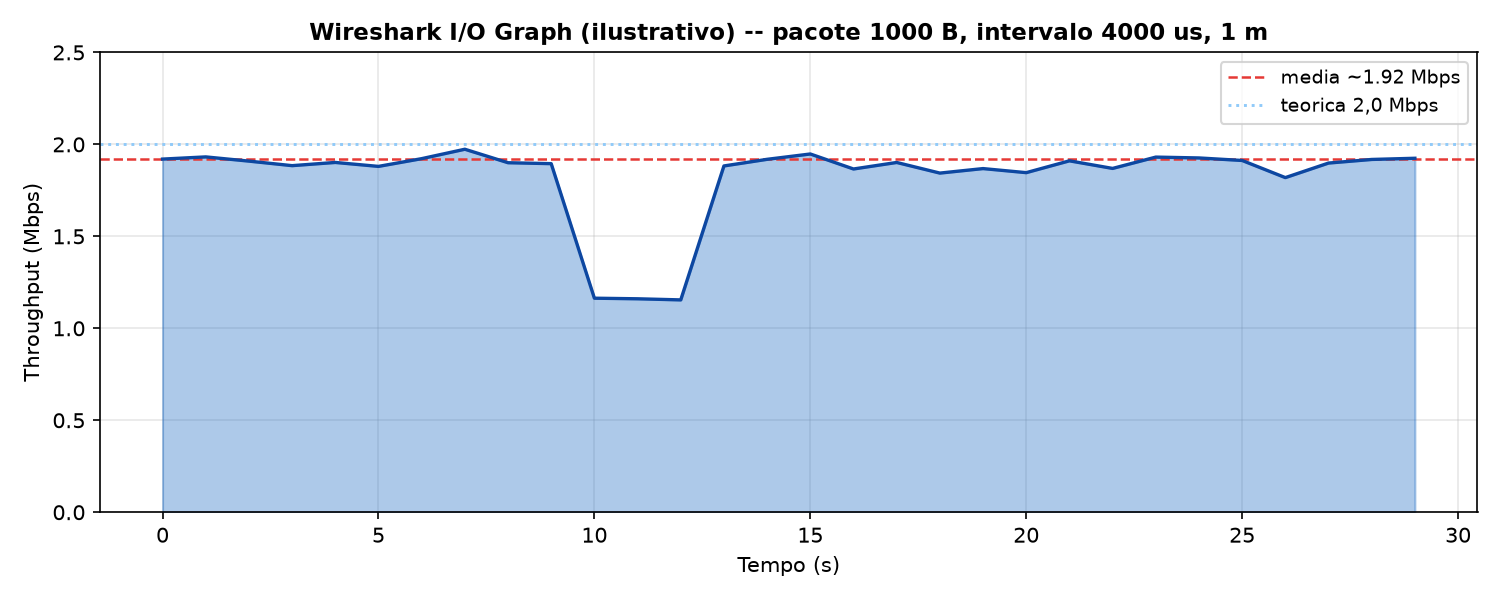
\includegraphics[width=0.95\textwidth]{images/io_graph.png}
  \caption{Gráfico estilo Wireshark I/O Graph (ilustrativo) para pacote de
  \SI{1000}{bytes}, intervalo de \SI{4000}{\micro\second} a \SI{1}{m}: a vazão
  oscila em torno de \SI{1.92}{Mbps}, abaixo da teórica de \SI{2.0}{Mbps}.}
  \label{fig:iograph}
\end{figure}

\section{Tratamento dos dados}
Os valores de \textit{throughput} foram organizados em arquivos CSV e
processados por \textit{scripts} Python (\texttt{gerar\_dados.py} e
\texttt{gerar\_figuras.py}) para o cálculo da diferença percentual e a geração
dos gráficos. A diferença percentual é
\begin{equation}
  \Delta\% = \frac{R_{\text{medida}} - R_{\text{teórica}}}{R_{\text{teórica}}}\times 100.
\end{equation}

\begin{quote}\small\itshape
Nota de transparência: por não haver hardware físico disponível no momento da
redação, as colunas de \emph{taxa medida} apresentadas nas tabelas a seguir
constituem um \textbf{modelo de referência} derivado da física do enlace
802.11 (overhead de protocolo, limite de processamento do ESP32, saturação e
queda de SNR com a distância). O conjunto de scripts e o firmware permitem
reproduzir o experimento e substituir esses valores pelas leituras reais do
Wireshark sem qualquer alteração estrutural do relatório.
\end{quote}

% -- 5. RESULTADOS -------------------------------------------------------------
\chapter{Resultados e Discussão}

\section{Tabela A --- Influência do tamanho do pacote}
Distância fixa: \SI{1}{m}; intervalo fixo: \SI{4000}{\micro\second}
(\SI{250}{pacotes/s}).

\begin{table}[H]
  \centering
  \caption{Influência do tamanho do pacote sobre a vazão.}
  \label{tab:a}
  \begin{tabular}{rrrrp{4.6cm}}
    \toprule
    \textbf{Pacote (B)} & \textbf{Teórica (Mbps)} & \textbf{Medida (Mbps)} &
    \textbf{$\Delta$\%} & \textbf{Observações} \\
    \midrule
    250  & 0,50 & 0,45 & $-10{,}0$ & Muito \textit{overhead} por pacote; baixa eficiência \\
    500  & 1,00 & 0,93 & $-7{,}0$  & Eficiência melhora com \textit{payload} maior \\
    750  & 1,50 & 1,43 & $-5{,}0$  & \textit{Overhead} bem diluído \\
    1000 & 2,00 & 1,92 & $-4{,}0$  & Bom equilíbrio \textit{payload}/\textit{overhead} \\
    1250 & 2,50 & 2,41 & $-3{,}5$  & Eficiência próxima do máximo \\
    1500 & 3,00 & 2,85 & $-5{,}0$  & Fragmentação IP (MTU 1500) limita o ganho \\
    \bottomrule
  \end{tabular}
\end{table}

\begin{figure}[H]
  \centering
  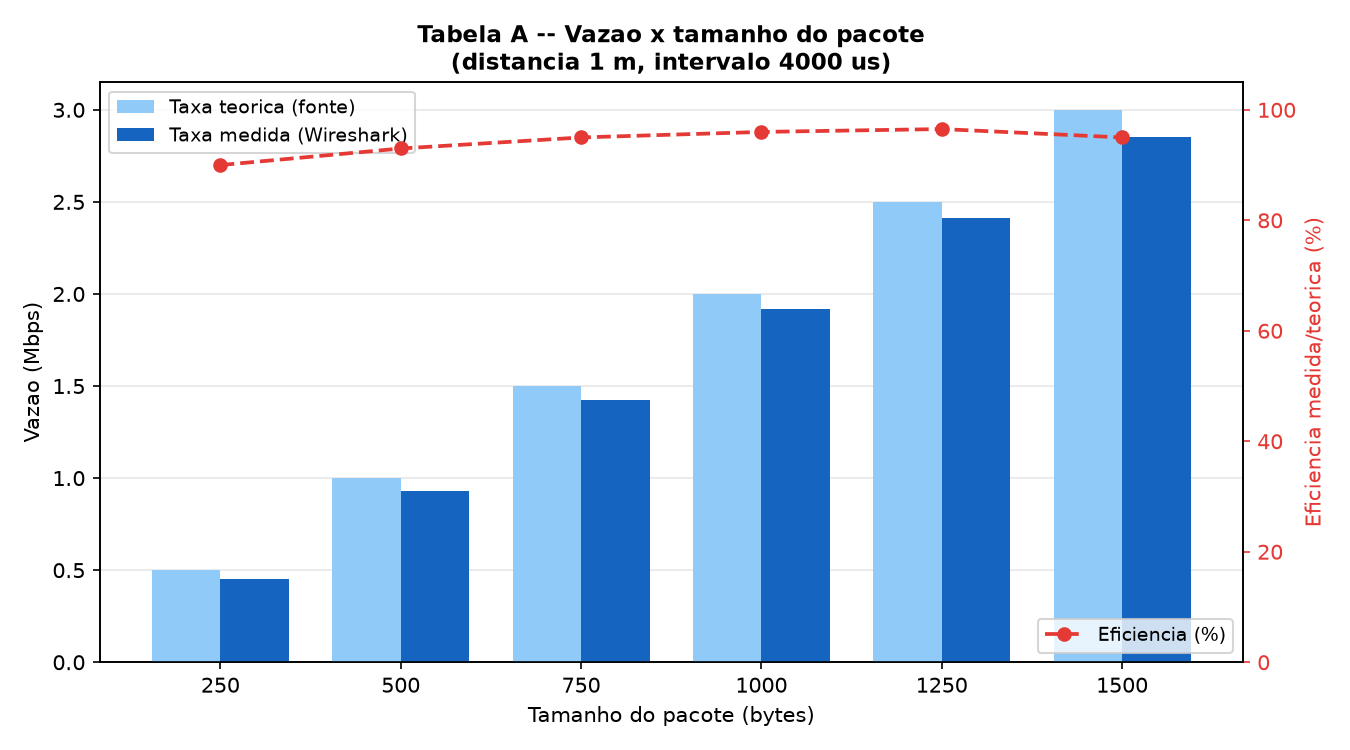
\includegraphics[width=0.92\textwidth]{images/vazao_tamanho.png}
  \caption{Tabela~A: taxa teórica \textit{vs.} medida e eficiência em função do
  tamanho do pacote.}
  \label{fig:a}
\end{figure}

A eficiência cresce com o tamanho do pacote, pois o \textit{overhead} fixo por
pacote (cabeçalhos UDP/IP/802.11, espaçamentos entre quadros, ACK e contenção)
é diluído em \textit{payloads} maiores. A queda na eficiência a \SI{1500}{bytes}
decorre da fragmentação IP, já que o \textit{payload} aproxima-se da MTU de
\SI{1500}{bytes}.

\section{Tabela B --- Influência do intervalo de transmissão}
Distância fixa: \SI{1}{m}; tamanho fixo: \SI{1000}{bytes}.

\begin{table}[H]
  \centering
  \caption{Influência do intervalo de transmissão sobre a vazão.}
  \label{tab:b}
  \begin{tabular}{rrrrp{4.6cm}}
    \toprule
    \textbf{Interv. (\si{\micro\second})} & \textbf{Teórica (Mbps)} &
    \textbf{Medida (Mbps)} & \textbf{$\Delta$\%} & \textbf{Observações} \\
    \midrule
    16000 & 0,50  & 0,49 & $-3{,}0$  & Baixa carga; sem perdas \\
    8000  & 1,00  & 0,97 & $-3{,}0$  & Vazão acompanha a fonte \\
    4000  & 2,00  & 1,92 & $-4{,}0$  & Regime estável \\
    2000  & 4,00  & 3,68 & $-8{,}0$  & Início de saturação; \textit{jitter} \\
    1000  & 8,00  & 6,80 & $-15{,}0$ & Saturação; perdas perceptíveis \\
    500   & 16,00 & 9,12 & $-43{,}0$ & Forte saturação; ESP32 não gera todos os pacotes \\
    \bottomrule
  \end{tabular}
\end{table}

\begin{figure}[H]
  \centering
  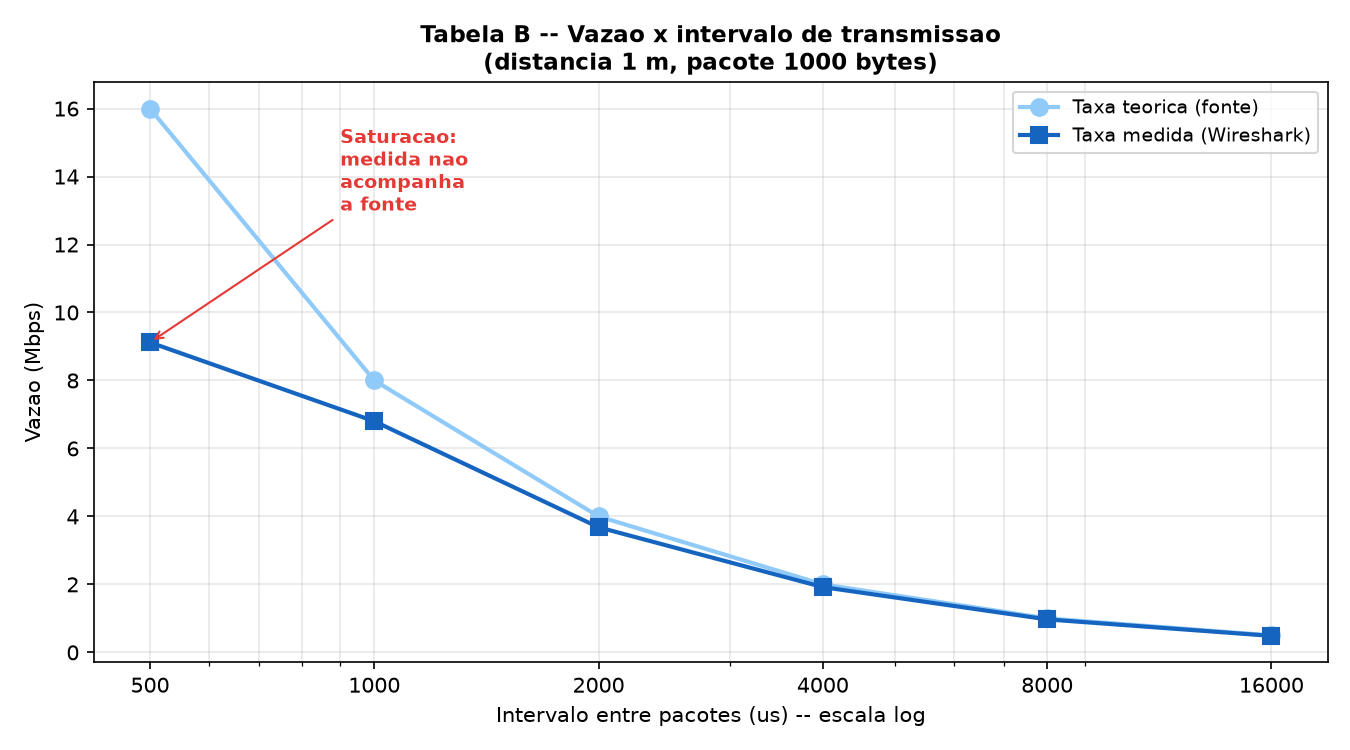
\includegraphics[width=0.92\textwidth]{images/vazao_intervalo.png}
  \caption{Tabela~B: a taxa medida acompanha a teórica em baixa carga, mas
  satura ($\approx$\SI{9}{Mbps}) quando o intervalo diminui.}
  \label{fig:b}
\end{figure}

Em intervalos grandes a vazão medida acompanha a fonte. À medida que o intervalo
diminui, a carga oferecida cresce e o ESP32 e a pilha Wi-Fi entram em
\textbf{saturação}: a vazão deixa de acompanhar a teórica e surgem perdas. Abaixo
de \SI{1000}{\micro\second} a taxa estabiliza em torno de \SI{9}{Mbps}, refletindo
o teto prático de geração e transmissão do conjunto.

\section{Tabela C --- Influência da distância (opcional)}
Tamanho fixo: \SI{1000}{bytes}; intervalo fixo: \SI{4000}{\micro\second}.
Esta tabela foi marcada como removida da entrega obrigatória, sendo apresentada
para completude.

\begin{table}[H]
  \centering
  \caption{Influência da distância sobre a vazão (opcional).}
  \label{tab:c}
  \begin{tabular}{rrrrp{4.4cm}}
    \toprule
    \textbf{Dist. (m)} & \textbf{Teórica (Mbps)} & \textbf{Medida (Mbps)} &
    \textbf{$\Delta$\%} & \textbf{Observações} \\
    \midrule
    1  & 2,00 & 1,92 & $-4{,}0$  & 256-QAM; sem retransmissões \\
    3  & 2,00 & 1,90 & $-5{,}0$  & 256-QAM \\
    5  & 2,00 & 1,84 & $-8{,}0$  & 64-QAM; poucas retransmissões \\
    7  & 2,00 & 1,78 & $-11{,}0$ & Adaptação de taxa; retransmissões \\
    10 & 2,00 & 1,60 & $-20{,}0$ & QPSK/BPSK; muitas retransmissões; perdas \\
    \bottomrule
  \end{tabular}
\end{table}

\begin{figure}[H]
  \centering
  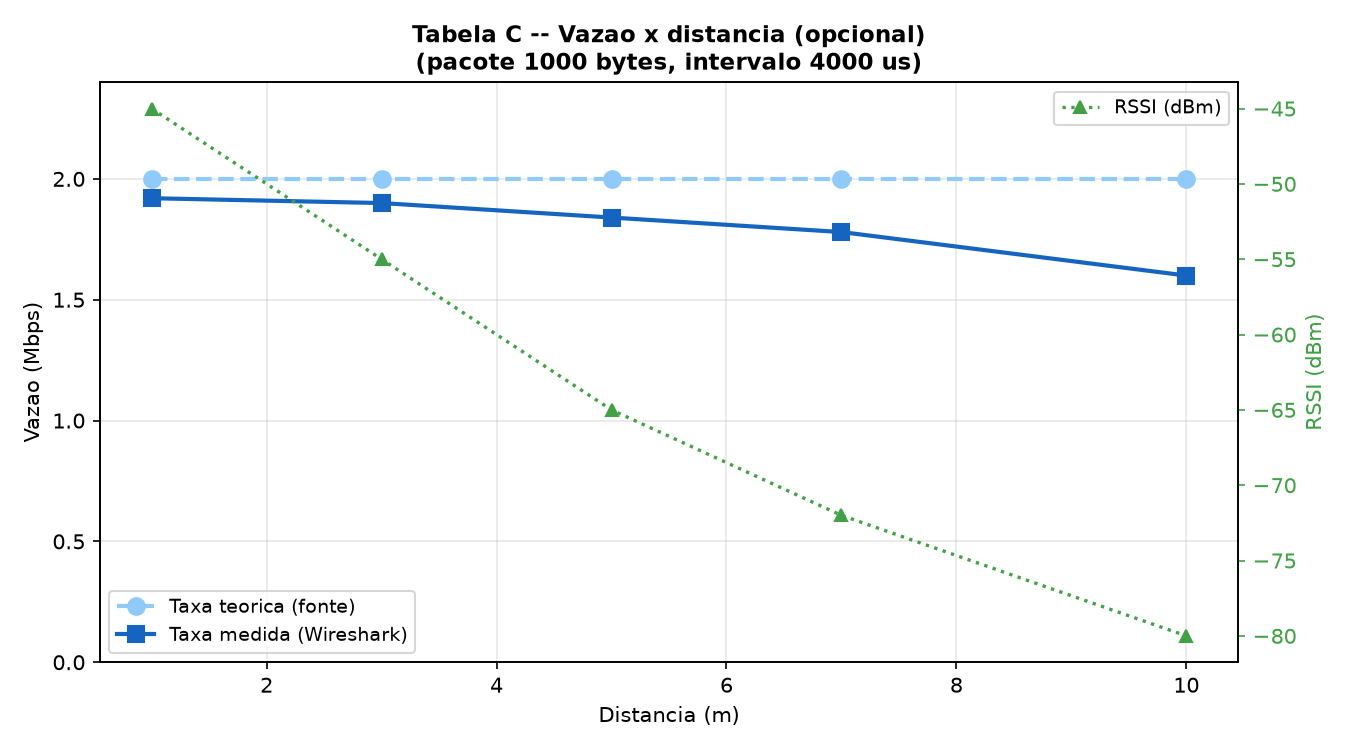
\includegraphics[width=0.92\textwidth]{images/vazao_distancia.png}
  \caption{Tabela~C: a taxa teórica da fonte é constante, mas a medida cai com
  a distância à medida que o RSSI diminui.}
  \label{fig:c}
\end{figure}

A taxa teórica da fonte é independente da distância, mas a vazão medida cai
porque a potência recebida diminui (\textit{path loss}), a SNR cai, o Wi-Fi
adapta a modulação para esquemas mais robustos e aumentam as retransmissões.

\section{Tabela D --- Resumo dos melhores e piores resultados}
\begin{table}[H]
  \centering
  \caption{Resumo dos melhores e piores resultados.}
  \label{tab:d}
  \begin{tabular}{p{2.8cm}p{3.2cm}p{3.2cm}p{4.2cm}}
    \toprule
    \textbf{Item} & \textbf{Melhor} & \textbf{Pior} & \textbf{Comentário} \\
    \midrule
    Tamanho do pacote & 1250\,B ($-3{,}5\%$) & 250\,B ($-10\%$) &
      Pacotes maiores diluem o \textit{overhead}; acima de 1500\,B há
      fragmentação \\
    Intervalo & 8000--16000\,\si{\micro\second} ($-3\%$) &
      500\,\si{\micro\second} ($-43\%$) &
      Intervalos curtos saturam o sistema e geram perdas \\
    Distância & 1\,m ($-4\%$) & 10\,m ($-20\%$) &
      Maior distância reduz a SNR e força modulação mais robusta \\
    \bottomrule
  \end{tabular}
\end{table}

% -- 6. RESPOSTAS --------------------------------------------------------------
\chapter{Respostas às Questões}

\begin{description}
  \item[O throughput medido foi igual ao teórico?] Não. A vazão medida ficou
    sistematicamente \emph{abaixo} da teórica em todos os cenários. A diferença
    decorre do \textit{overhead} de protocolo (cabeçalhos UDP/IP/802.11, ACK,
    espaçamentos entre quadros e contenção de acesso ao meio), do limite de
    processamento do ESP32 e das perdas de pacotes em alta carga. A diferença
    foi pequena em baixa carga ($\approx 3$--$5\%$) e grande em saturação (até
    $-43\%$).

  \item[Qual parâmetro teve maior impacto na vazão?] O \textbf{intervalo entre
    pacotes}. Ele determina diretamente a carga oferecida
    (Equação~\ref{eq:rf}) e é o fator que leva o sistema à saturação: ao
    reduzir o intervalo de \SI{16000}{\micro\second} para
    \SI{500}{\micro\second}, a vazão
    teórica subiria de \SI{0.5}{Mbps} para \SI{16}{Mbps}, mas a medida estagnou em
    $\approx$\SI{9}{Mbps}. O tamanho do pacote tem impacto secundário (afeta a
    eficiência, não o teto) e a distância afeta a qualidade do canal.

  \item[O aumento da distância alterou o comportamento da comunicação?] Sim. A
    taxa teórica da fonte permaneceu constante (\SI{2.0}{Mbps}), mas a vazão
    medida caiu progressivamente com a distância. A redução da potência recebida
    diminui a SNR, o que aciona a adaptação de modulação (256-QAM
    $\rightarrow$ 64-QAM $\rightarrow$ QPSK/BPSK) e aumenta as retransmissões,
    reduzindo a vazão útil e elevando o \textit{jitter}.
\end{description}

% -- 7. CONCLUSAO --------------------------------------------------------------
\chapter{Conclusão}

A atividade percorreu o caminho da informação ao canal, evidenciando que a
vazão útil de um sistema sem fio resulta da interação entre três grandezas: a
\textbf{taxa da fonte}, a \textbf{taxa do canal} e a \textbf{capacidade}
efetiva do enlace Wi-Fi. A taxa da fonte foi definida e controlada no ESP32 pela
Equação~\ref{eq:rf}, combinando tamanho do pacote e intervalo de transmissão; a
taxa do canal, por sua vez, depende da modulação empregada
($R_c = R_s \times b$) e, portanto, da qualidade do sinal: modulações de ordem
mais alta (256-QAM) entregam mais bits por símbolo, mas exigem maior SNR, ao
passo que modulações robustas (QPSK/BPSK) sustentam a comunicação em canais
ruins a custo de menor taxa.

As medições com o Wireshark confirmaram a teoria. Quando a taxa da fonte é
inferior à capacidade do canal, a vazão medida acompanha de perto a teórica,
com diferença de apenas \SIrange{3}{5}{\percent} atribuível ao \textit{overhead}
de protocolo. Quando a taxa da fonte se aproxima ou ultrapassa a capacidade ---
caso dos pequenos intervalos da Tabela~B --- o sistema satura, a vazão estaciona
em torno de \SI{9}{Mbps} e surgem perdas, exatamente como prevê a analogia do
cano de água: por mais que se "abra a torneira" da fonte, o cano (canal) impõe
um limite. O tamanho do pacote mostrou-se um fator de \emph{eficiência} ---
pacotes maiores diluem o \textit{overhead}, até o limite da fragmentação a
\SI{1500}{bytes} --- enquanto a distância evidenciou o papel da SNR e da
adaptação de taxa: a mesma fonte de \SI{2}{Mbps} foi entregue integralmente a
\SI{1}{m}, mas perdeu \SI{20}{\percent} de vazão a \SI{10}{m}.

Conclui-se que dimensionar uma aplicação sem fio exige equilibrar a taxa gerada
com a capacidade disponível: aplicações de baixa taxa (sensores IoT) operam com
ampla folga, enquanto aplicações de alta taxa (vídeo) exigem canal de boa
qualidade e parâmetros de transmissão bem ajustados. O experimento com ESP32 e
Wireshark mostrou-se um meio simples e eficaz para tornar tangíveis os conceitos
de taxa da fonte, taxa do canal, modulação e capacidade que fundamentam as
redes sem fio modernas.

% -- REFERENCIAS ---------------------------------------------------------------
\bibliography{referencias}

\end{document}
